\documentclass{article}
\usepackage[utf8]{inputenc}
\usepackage{graphicx}
\usepackage{subcaption}
\usepackage[bottom=0.5in,top=0.5in,right=1in,left=1in]{geometry}
\usepackage[section]{placeins}
\usepackage{float}
\title{Experiment 5}
\author{Nitish Kumar Thakur \\ 21531010 }
\date{31 August, 2021}

\begin{document}

\maketitle

\section{Objective}
1.Determine the lock range and capture range of the PLL IC-565 \par
2.Demodulate FM signal using the PLL IC-565
 
 \section{Components and Equipment Required}                    
 IC-565 PLL IC*IC-8038 *DSO *Power supply (variable)*connecting wire *Breadboard *probes *Resistance *DSO *Function generator
 
\section{Theory}

\subsection{Phase lock loop}
Phase-locked loop is a feedback control system that automatically adjusts the phase of a locally generated signal to match the phase of an input signal. PLLs operate by producing an oscillator frequency to match the frequency of an input signal. In this locked condition, any slight change in the input signal first appears as a change in phase between the input signal and the oscillator frequency. This phase shift then acts as an error signal to change the frequency of the local PLL oscillator to match the input signal. The locking-onto-a-phase relationship between the input signal and the local oscillator accounts for the name phase-locked loop.
\begin{figure*}[h]
	\centering
	\includegraphics[scale=0.65]{3.png}
	\caption{PLL}
	\label{FBD}
\end{figure*}
if we analyse the figure there is basically 4 Block.
\subsubsection{Phase Detector}
A phase detector is nothing but a comparator.It performs a comparison of two frequency component fed at its input and generates a dc voltage.This generated voltage is proportional to the difference in phase of the two frequencies.

\subsubsection{Low pass filter}
The output of the phase detector is provided to a low pass filter.It eliminates the high-frequency component and noise from the output of the comparator.This low-frequency dc voltage signal is then provided to a dc  amplifier which amplifies the signal level.This amplified signal is then provided to the VCO

\subsubsection{Voltage Controlled Oscillator}
Voltage-controlled oscillator is electronic oscillator the work of VCO is when we give variable voltage in VCO it generates varying frequency curve(Linear).This thing shown in below Figure
The output of LPF acts as a control signal to the VCO.The VCO generates a dc signal, the amplitude of which is  proportional to the amplitude of output of LPF.Here the adjustment in the output frequency of VCO is made until it shows equivalency with the input signal frequency.

\begin{figure*}[h]
	\centering
	\includegraphics[scale=0.6]{22.png}
	\caption{Voltage-controlled oscillator}
	\label{FBD}
\end{figure*}
\subsubsection{Dc Amplifier}
Amout of gain we getting is very-very less so we use DC amplifier.

Phase Lock Loop basically work in two mode \par
1.Capture range\par2.Lock range\par

\textbf{1.Capture range}\par
The process of adjusting the VCO frequency and holding it to incoming signals frequency is called capture.The minimum and maximum input frequencies to which the loop can move the VCO as it captures an input signal is called the capture range.The segments of the capture range above and below fo are called the pull-in range.The pull-in ranges are not necessarily symmetrical.\par
\par

\textbf{2.Lock range} \par
If the input frequency has moved so far that any further change will cause the control signal to move back and the VCO frequency away from the input signal.The loop is no longer locked and the input and VCO frequencies are no longer the same.The range of input frequencies between the value at which the loop is locked is called the loop’s lock range.The lock range above and below f0 are called the loop’s hold ranges.The lock range is not always centered on f0

\begin{figure}[h]
  \begin{subfigure}[b]{0.5\textwidth}
    \includegraphics[width=\textwidth]{10.jpg}
    \caption{Capture range/ Lock range}
    \label{fig:1}
  \end{subfigure}
  %
  \begin{subfigure}[b]{0.4\textwidth}
    \includegraphics[width=\textwidth]{11.png}
    \caption{Free running Frequency of VCO calculatio}
    \label{fig:2}
  \end{subfigure}
\end{figure}

\subsection{IC LM565 Pin diagram/ block diagram}


\begin{figure}[h]
  \begin{subfigure}[b]{0.5\textwidth}
    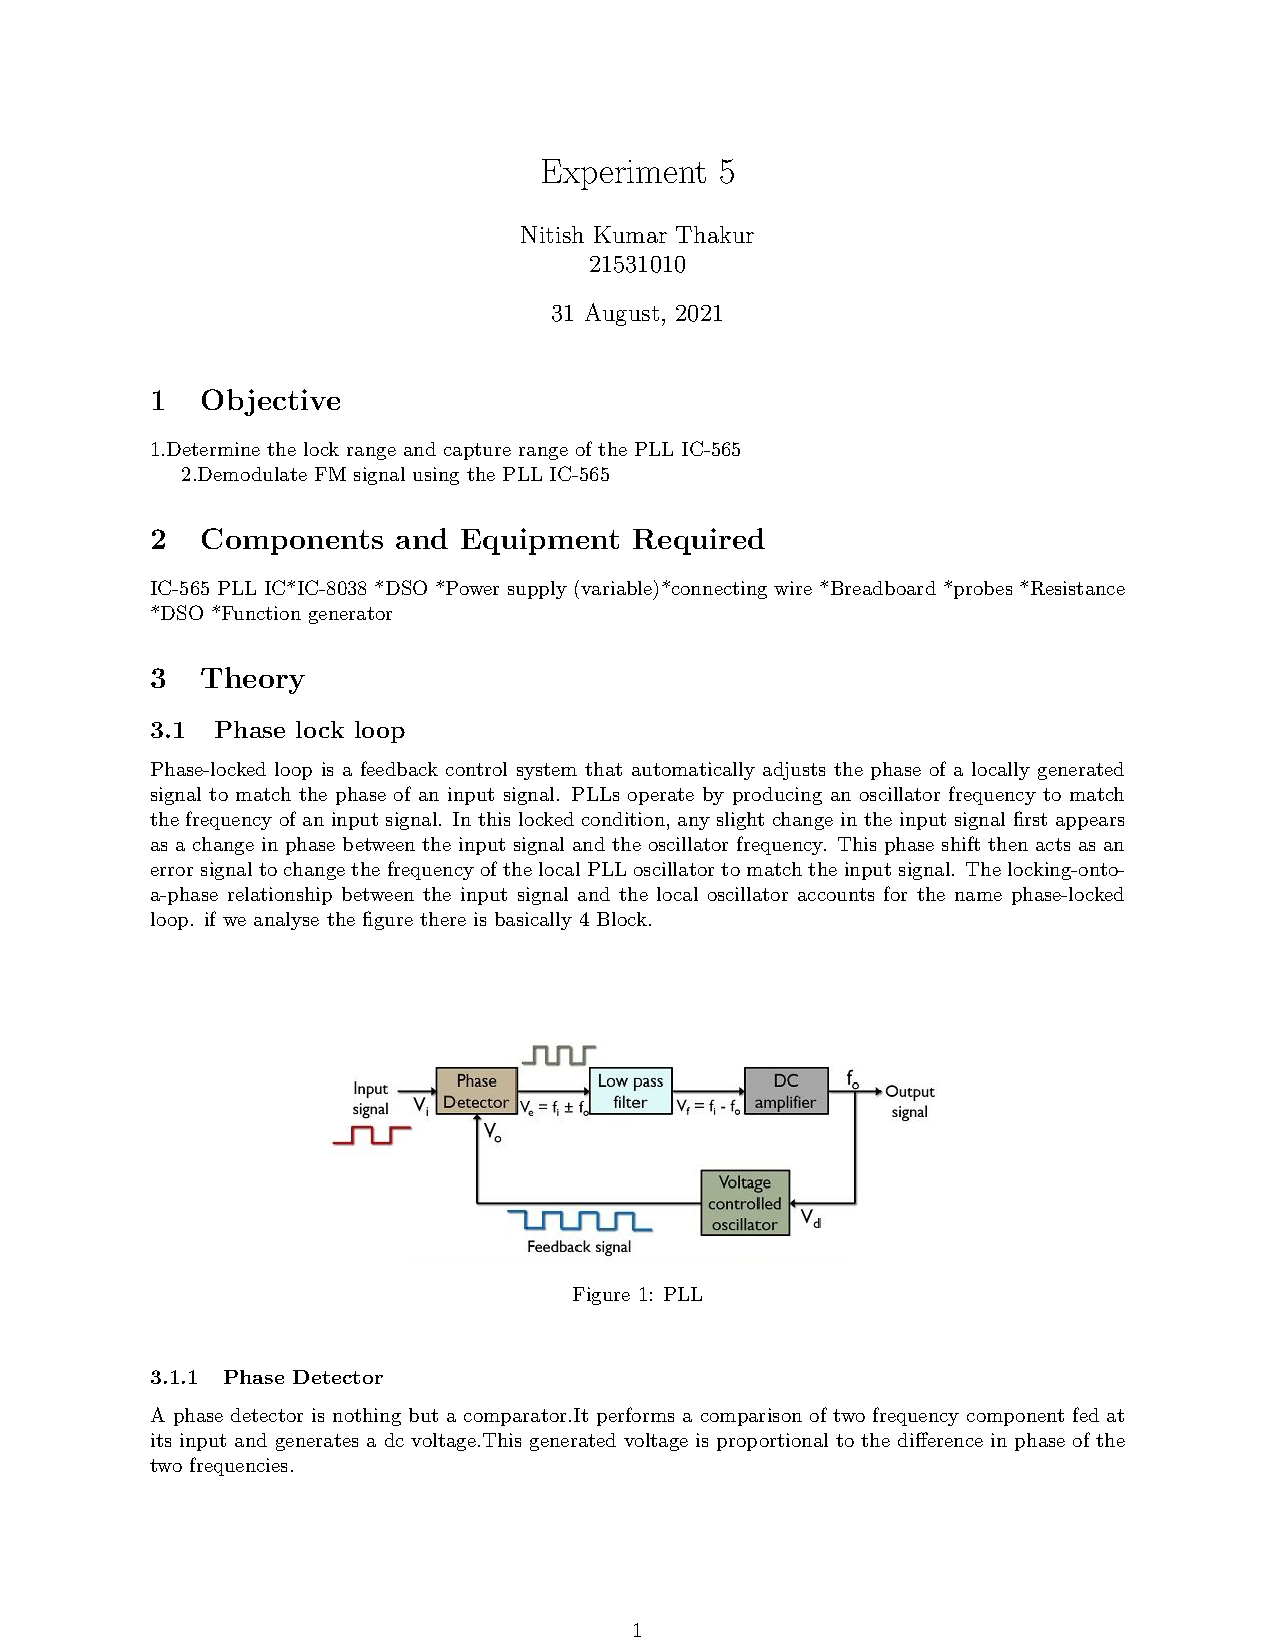
\includegraphics[width=\textwidth]{5.png}
    \caption{ IC LM-565 Pin diagram}
    \label{fig:1}
  \end{subfigure}
  %
  \begin{subfigure}[b]{0.4\textwidth}
    \includegraphics[width=\textwidth]{6.png}
    \caption{Block diagram of IC LM-565}
    \label{fig:2}
  \end{subfigure}
\end{figure}
\subsection{Frequency Demodulation}

\begin{figure*}[h]
	\centering
	\includegraphics[scale=0.6]{freq demod.png}
	\caption{Frequency Demodulation}
	\label{FBD}
\end{figure*}
Circuit Diagram
\begin{figure*}[ht]
	\centering
	\includegraphics[scale=0.5]{101.png}
	\caption{Circuit diagram of  demodulation}
	\label{FBD}
\end{figure*}















\section{Observation/Results}

\subsection{Free Running frequency}

\begin{figure}[ht]
  \begin{subfigure}[b]{0.5\textwidth}
    \includegraphics[width=\textwidth]{1.png}
    \caption{ Circuit on BreadBoard}
    \label{fig:1}
  \end{subfigure}
  %
  \begin{subfigure}[b]{0.5\textwidth}
    \includegraphics[width=\textwidth]{1.1.png}
    \caption{Free running Frequency}
    \label{fig:2}
  \end{subfigure}
\end{figure}

Output frequency in case of free running VCO is-9.954Khz.This frequency almost equal to incoming signal.After this our aim to select proper value of R and C\par
\begin{figure*}[ht]
	\centering
	\includegraphics[scale=0.6]{11.png}
	\caption{Equation for calculation of R and C}
	\label{FBD}
\end{figure*}

R1=10Kohm(9.954Kohm By multimeter),C1=3.3 nF,C2=5nF\par 
if R=10Kohm-fo=9.09Khz\par
R=9.54Khz for fo=9.529Khz\par

After This we give input signal.frequency=6.5Khz and see what's the vco output.VCO output frequency is f=6.499Khz,in lower figure.
\begin{figure*}[ht]
	\centering
	\includegraphics[scale=0.6]{input.png}
	\caption{Input at pin-2/and VCO output}
	\label{FBD}
\end{figure*}

After this we want to see in which range it is phase lock.so we first increase the frequency slowly and see where it is lock.it is known forward locking range.

\begin{figure}[h]
  \begin{subfigure}[b]{0.4\textwidth}
    \includegraphics[width=\textwidth]{forward lock .png}
    \caption{forward lock range start at f=6.3Khz}
    \label{fig:1}
  \end{subfigure}
  %
  \begin{subfigure}[b]{0.4\textwidth}
    \includegraphics[width=\textwidth]{lock range comp.png}
    \caption{lock range end at f=14.9Khz}
    \label{fig:2}
  \end{subfigure}
\end{figure}








Now we go for backward direction.Backward lock range start at f=14 Khz.Backward lock range stop at f=6.2Khz

so we take common data for capture range i.e 6.3khz-14khz.\par
and Lock range is 6.2khz-14khz.
if we calculate theoretically then\par
 Fl=7.962khz  \par
 Fc=8.39Khz  \par
so we use pll in this range to demodulate our frquency modulated signal.

VCO characteristic

\begin{figure*}[h]
	\centering
	\includegraphics[scale=0.4]{output after demod.png}
	\caption{Modulated signal output}
	\label{FBD}
\end{figure*}

This is final output after demodulation

\begin{figure*}[h]
	\centering
	\includegraphics[scale=0.35]{final.png}
	\caption{Final demodulated signal}
	\label{FBD}
\end{figure*}

\section{Conclusion/Sources of error}
 If we observe output that means demodulated signal we did not get perfect output like input sinusoidal.because PLL output is square waveform which is not perfect(Gibb's phenomena)\par when we observe the demodulated signal frequency it is 712.3 Hz.which is nearer to original Message signal\par
 also when we calculate theoretically Lock range and capture range we found lock range is less then capture range.but we know lock range always higher then capture range.this problem i think due to problem with resistor and capacitor,which is not perfect.
 
 
\end{document}
